%    (at your option) any later version.
%
%    This program is distributed in the hope that it will be useful,
%    but WITHOUT ANY WARRANTY; without even the implied warranty of
%    MERCHANTABILITY or FITNESS FOR A PARTICULAR PURPOSE.  See the
%    GNU General Public License for more details.
%
%    You should have received a copy of the GNU General Public License
%    along with this program.  If not, see <http://www.gnu.org/licenses/>.
%========================================
%	苏州大学本科生论文LaTeX模板
%	2010年 05月 29日 星期六 19:47:22 CST
%	By telive
%	Email:	tellive@gmail.com
%========================================

\documentclass[a4paper, 12pt]{article}

%    it under the terms of the GNU General Public License as published by
%    the Free Software Foundation, either version 3 of the License, or
%    (at your option) any later version.
%
%    This program is distributed in the hope that it will be useful,
%    but WITHOUT ANY WARRANTY; without even the implied warranty of
%    MERCHANTABILITY or FITNESS FOR A PARTICULAR PURPOSE.  See the
%    GNU General Public License for more details.
%
%    You should have received a copy of the GNU General Public License
%    along with this program.  If not, see <http://www.gnu.org/licenses/>.

%========================================
%	苏州大学论文LaTeX模板
%	2010年 05月 29日 星期六 19:47:22 CST
%	By telive
%	Email:	tellive@gmail.com
%========================================

%========================================
%		Packages used in this template
\usepackage[BoldFont, SlantFont]{xeCJK}			% 中文支持
\usepackage{pdfpages}		% 插入pdf
\usepackage{graphicx}		% 图形支持
\usepackage{epsfig}
\usepackage{titletoc}
\usepackage{subfigure, float}
\usepackage{indentfirst}
\usepackage{calc}
\usepackage{amssymb, amsmath}	% 数学符号
\usepackage{fancybox}		% 方框文字
\usepackage{wrapfig}		% 图片文字环绕
\usepackage{fancyhdr}		% 页眉设置
\usepackage{cite}			% 引用文献
\usepackage{indentfirst}	% 首行缩进
\usepackage[colorlinks,linkcolor=blue,citecolor=blue]{hyperref}			% 让 TOC 支持超链接
\usepackage[top=3.3cm,bottom=2.7cm,left=2.75cm,right=2.75cm]{geometry}  %设置页边距(学校的要求)
\usepackage{fontspec}
\usepackage{caption}
\usepackage{color}
\usepackage{array}
\usepackage{mhchem}
\usepackage{titlesec}
\usepackage{ctex}
\usepackage{listings}
\usepackage{color}
\newcommand{\PreserveBackslash}[1]{\let\temp=\\#1\let\\=\temp}
\newcolumntype{C}[1]{>{\PreserveBackslash\centering}p{#1}}
\newcolumntype{R}[1]{>{\PreserveBackslash\raggedleft}p{#1}}
\newcolumntype{L}[1]{>{\PreserveBackslash\raggedright}p{#1}}

%========================================
%		Settings
\setmainfont{Times New Roman}
\setCJKmainfont{SimSun}					% 中文默认字体设置为宋体
\setCJKfamilyfont{Heiti}{SimHei}		% Use \CJKfamily{Heiti} where you need.
\setCJKfamilyfont{Songti}{SimSun} 		% Use \CJKfamily{Songti} where you need.
% \setCJKfamilyfont{Kaiti}{simkai.ttf} 	% Use \CJKfamily{Kaiti} where you need.
\setlength{\parindent}{2em}				% 首行缩进,2字符
\numberwithin{equation}{section}   		% 使公式标号为 3.1 的形式

\newcommand\Heiti{\CJKfamily{Heiti}}
\newcommand\Songti{\CJKfamily{Songti}}
\newcommand\Kaiti{\CJKfamily{Kaiti}}

%========================================
%		Redefine commands
\renewcommand\abstractname{\Large \bfseries \Songti 摘\ 要}	% 摘要
\renewcommand{\figurename}{\Songti 图} 					     % 图
\renewcommand{\tablename}{\Songti 表}           			     % 表
\renewcommand\refname{\Songti 参考文献}				 	      % 参考文献
\renewcommand\contentsname{\centerline{\Songti 目录}}	        % 目录居中
\renewcommand{\today}{\number\year 年 \number\month 月 \number\day 日}	%中文日期
%\renewcommand{\theequation}{\arabic{chapter}-\arabic{equation}}

%========================================
%		Header Settings

\pagestyle{fancy}
\pagenumbering{arabic}
\titlecontents{section}
	[2.5cm]
	{\CJKfamily{Heiti}}
	{\contentspush{第\thecontentslabel\ 章\quad}}
	{}
	{\titlerule*[0.5pc]{$\cdot$}\contentspage\hspace*{2cm}}
\titlecontents{subsection}
	[4cm]
	{\normalsize}
	{\contentslabel{2.5em}}
	{}
	{\titlerule*[0.5pc]{$\cdot$}\contentspage\hspace*{2cm}}
\titlecontents{subsubsection}
	[4.2cm]
	{\normalsize}
	{\contentslabel{2.5em}}
	{}
	{\titlerule*[0.5pc]{$\cdot$}\contentspage\hspace*{2cm}}

\chead{ \footnotesize  \Songti 苏州大学本科生毕业设计(论文)}	% 页眉中部
\lhead{}		% 页眉左部,设为空
\rhead{}		% 页眉右部,设为空

%========================================
%		Caption settings

\DeclareCaptionFont{kaiti}{\Kaiti}
\DeclareCaptionFont{bfheiti}{\bf\Heiti}
\captionsetup{font=small, format=plain, labelfont=bfheiti,
	textfont=kaiti, justification=raggedright,
	singlelinecheck=false
}
\titleformat{\section}{\centering\Large\bfseries}{第\thesection\,章}{1em}{}

\newcommand{\enabstractname}{ \bfseries \Songti Abstract}
\newcommand{\cnabstractname}{ \bfseries \Songti 摘\ 要}
\newenvironment{enabstract}{%
  \par\small
  \noindent\mbox{}\hfill{\bfseries \enabstractname}\hfill\mbox{}\par
  \vskip 2.5ex}{\par\vskip 2.5ex}
\newenvironment{cnabstract}{%
  \par\small
  \noindent\mbox{}\hfill{\bfseries \cnabstractname}\hfill\mbox{}\par
  \vskip 2.5ex}{\par\vskip 2.5ex}


 
  
  \definecolor{dkgreen}{rgb}{0,0.6,0}
  \definecolor{gray}{rgb}{0.5,0.5,0.5}
  \definecolor{mauve}{rgb}{0.58,0,0.82}
  
  \lstset{frame=tb,
	language=Python,
	aboveskip=3mm,
	belowskip=3mm,
	showstringspaces=false,
	columns=flexible,
	basicstyle={\small\ttfamily},
	numbers=none,
	numberstyle=\tiny\color{gray},
	keywordstyle=\color{blue},
	commentstyle=\color{dkgreen},
	stringstyle=\color{mauve},
	breaklines=true,
	breakatwhitespace=true,
	tabsize=3
  }


\begin{document}
%\pagenumbering{arabic}

%================== 封面 =================

\includepdf{cover.pdf}
\thispagestyle{empty}
\newpage


\includepdf{保密协议1.pdf}
\thispagestyle{empty}
\newpage

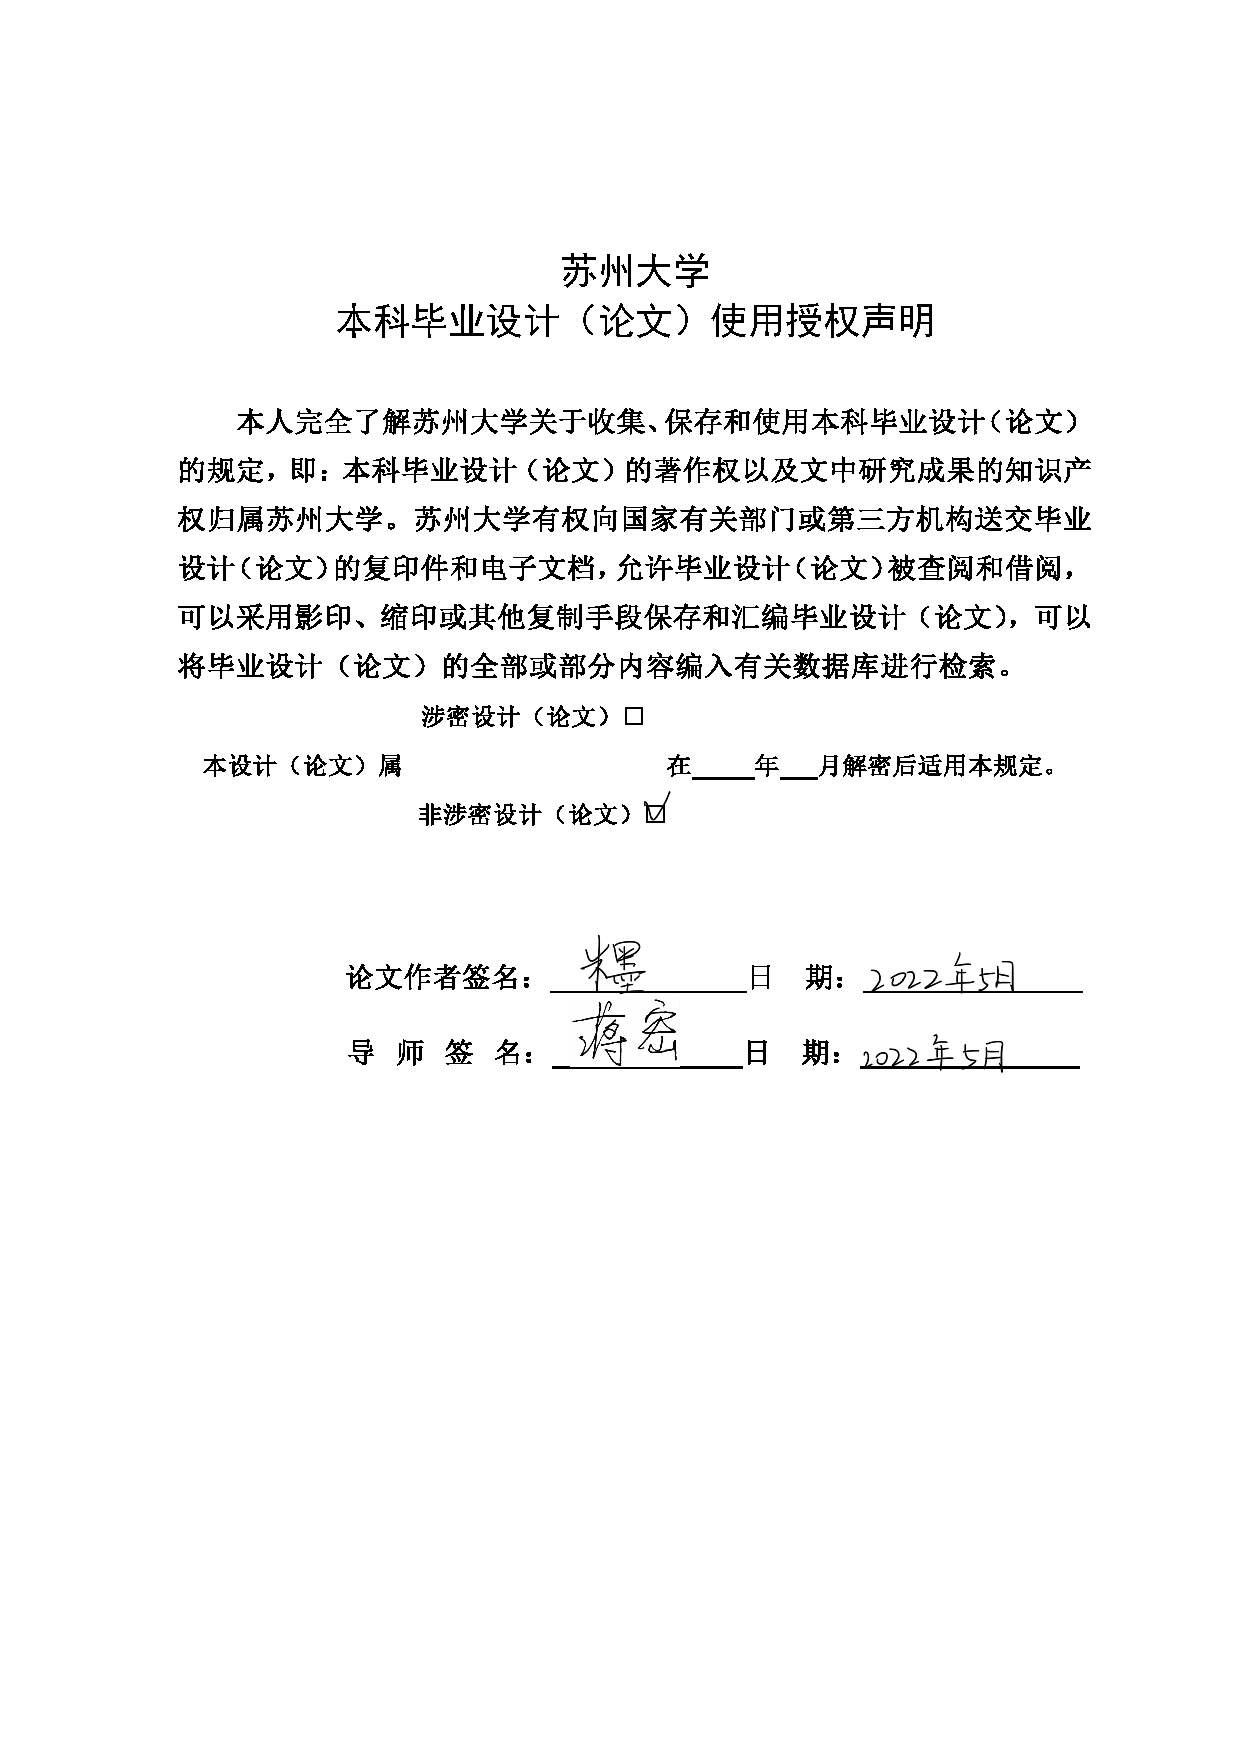
\includepdf{保密协议2.pdf}
\thispagestyle{empty}
\newpage


%================== 中英文摘要 ============
% A 中英文摘要、关键词 (从本页开始编页码)
\begin{center}
    \bf \Large\Heiti{重费米子物理的实验和理论研究进展}
\end{center}
\vskip1.5em
\begin{cnabstract}
		% 在目录中显示摘要
%========================================

重费米子材料是一种强关联电子统,最近出现多个不等价位点的化合物如\ce{Ce3(Pd/Pt)In11},其拥有两个不等位点Ce1和Ce2,其中一个Ce位点提供超导性,另一个Ce位点提供反铁磁性。针对这种系统我们利用DQMC构建模型,进行分析研究,研究得到一些初步的结果,本文的主要任务为分析程序的编写。
\\
\textbf{关键词}: \ \ 重费米子;强关联系统;量子蒙特卡罗计算;反铁磁性;超导态
\end{cnabstract}

%========================================
% 英文摘要

\vskip2em
\begin{center}
    \bf \Large\Heiti{Advances in Experimental and Physical Research of Heavy Fermion Physics}
\end{center}
\vskip1.5em
\begin{enabstract}
    Heavy fermion material is a strongly correlated electron system. Recently, compounds with multiple unequal sites have appeared, such as \ce{Ce3(Pd/Pt)In11}, which has two unequal sites Ce1 and Ce2, one of which is Ce One site provides superconductivity and the other Ce site provides antiferromagnetism. For this kind of system, we use DQMC to build a model, conduct analysis and research, and get some preliminary results. The main task of this paper is to program the analysis program.

    
\textbf{keywords}: \ \ Heavy Fermion; Strong connection system%corealtion; 
quantum Metor Carlo; antiferromagnetic; superconductivity;
\end{enabstract}  

\thispagestyle{empty}
\newpage

%================== 目录 =================
% B 目录
\tableofcontents
\thispagestyle{empty}
\newpage

%================== 前言  ================
% C 前言
% \pagenumbering{arabic}

\section{绪论}
\subsection{研究背景}
重费米行为由K.Andres,J.E.Graebner和H.R.Ott在1975年发现,他们观察到\ce{CeAl_3}中线性比热容
变化很大。在对掺杂超导体的研究中得出结论,一种材料中存在局域磁矩和超导态是不相容的,但是
在1979年,Frank Steglich等人在\ce{CeCu_2Si_2}中发现了重费米子的超导性。H.von Löhneysen等
人于1994年在重费米子化合物的相图中发现了量子临界点和非费米液体行为,导致人们对这些化合物
的研究产生了新的兴趣。另一个实验突破是(由Gil Lonzarich小组证明)重费米子中的量子临界性
可能是非常规超导性的原因。

常规超导现象的微观解释由Bardeen等人于1957年完成即BCS理论。而电阻极小值现象经过30多年的研究,最
终确定与金属杂质的存在由直接关联,并发现电阻在低温下呈现对数增长的行为。1964年,日本物理学家Kondo
借助微扰论方法处理电子和磁性杂质的相互作用,发现自旋反转散射过程会对电阻率产生正比于$-logT$的贡献,
进而与声子散射的$T^5$贡献相结合,可以在理论上解释稀磁合金的电阻极小现象。这一散射过程称为Kondo散射。
在微观图像上,受到超导现象中自旋相反的电子配对形成自旋相反的束缚态,被称为Konde单态。Konde效应
由一个特征温标来刻画,$T_K ~ \rho^{-1}e^{-1/J \rho_0}$,简称Kondo温度,其中J为磁性杂质遇到导带电子自旋的耦合强度,$\rho_0$为费米面上电子态密度。低于$T_K$时,微扰论失效,电阻率不再遵循$-logT$的行为。



\subsection{研究目的与意义}
\subsubsection{研究目的}
重费米子材料在当前的科学研究中发挥着重要作用,但是作为研究非常规超导、非费米液体行为和量子
临界性的原型材料,重费米子化合物中局域磁矩和传导电子之间的实际相互作用仍未完全了解,并且是
正在进行的研究主题。

\subsubsection{研究意义}



\subsection{研究内容与方法}



\subsubsection{研究内容}


\subsubsection{研究方法}


\subsection{研究思路}

% \newpage

%=================== 论文正文 =============
% D 论文正文
\pagenumbering{arabic}
\section{绪论}
\subsection{研究背景}
重费米行为由K.Andres,J.E.Graebner和H.R.Ott在1975年发现,他们观察到\ce{CeAl_3}中线性比热容
变化很大。在对掺杂超导体的研究中得出结论,一种材料中存在局域磁矩和超导态是不相容的,但是
在1979年,Frank Steglich等人在\ce{CeCu_2Si_2}中发现了重费米子的超导性。H.von Löhneysen等
人于1994年在重费米子化合物的相图中发现了量子临界点和非费米液体行为,导致人们对这些化合物
的研究产生了新的兴趣。另一个实验突破是(由Gil Lonzarich小组证明)重费米子中的量子临界性
可能是非常规超导性的原因。

常规超导现象的微观解释由Bardeen等人于1957年完成即BCS理论。而电阻极小值现象经过30多年的研究,最
终确定与金属杂质的存在由直接关联,并发现电阻在低温下呈现对数增长的行为。1964年,日本物理学家Kondo
借助微扰论方法处理电子和磁性杂质的相互作用,发现自旋反转散射过程会对电阻率产生正比于$-logT$的贡献,
进而与声子散射的$T^5$贡献相结合,可以在理论上解释稀磁合金的电阻极小现象。这一散射过程称为Kondo散射。
在微观图像上,受到超导现象中自旋相反的电子配对形成自旋相反的束缚态,被称为Konde单态。Konde效应
由一个特征温标来刻画,$T_K \sim \rho^{-1}e^{-1/J \rho_0}$,简称Kondo温度,其中J为磁性杂质遇到导带电子自旋的耦合强度,$\rho_0$为费米面上电子态密度。低于$T_K$时,微扰论失效,电阻率不再遵循$-logT$的行为。

重费米子材料在当前的科学研究中发挥着重要作用,但是作为研究非常规超导、非费米液体行为和量子
临界性的原型材料,重费米子化合物中局域磁矩和传导电子之间的实际相互作用仍未完全了解,并且是
正在进行的研究主题。
我们利用dqmc(Determinant Quantum Monte Carlo),对\ce{Ce3PdIn11}进行模拟。

\subsection{背景理论}
\subsubsection{量子蒙特卡洛}
DQMC非常适合高温下对强关联系统的模拟。强关联系统意味着量子粒子(例如电子)无法用独立电子近似描述(类似于密度泛函理论和能带结构计算)。一个著名的例子就是高温超导$T_C$的计算。

DQMC主要用来计算有限温度的费米子系统。在实际运作过程中,其中只有二费米子部分。DQMC将求Trace转化为了求矩阵的行列式。例如:
$$Tr[e^{- \sum_{i,j}\widehat{c}^\dagger_i A_{i,j}\widehat{c}_j}]=Det[\textbf{1}+e^{-\textbf{A}}]$$
其中$A_{i,j}$为矩阵A的元素,可以看到将求Trace转为求一个单位矩阵\textbf{1}加上矩阵$e^{-\textbf{A}}$。
对于此证明,将e指数上的部分进行对角化,Trace即为对于$n_i=0,1$的可能性求和:
$$
\operatorname{Tr}\left[e^{-\sum_{i, j} \hat{c}_{i}^{\dagger} A_{i, j} \hat{c}_{j}}\right]=\operatorname{Tr}\left[e^{-\sum_{k} \epsilon(k) \hat{c}_{k}^{\dagger} \hat{c}_{k}}\right]=\Pi_{k} \operatorname{Tr}\left[e^{-\epsilon(k) \hat{c}_{k}^{\dagger} \hat{c}_{k}}\right]=\Pi_{k}\left[1+e^{-\epsilon(k)}\right]
$$
上述等式显然成立。
对于上式推广:
$$
e^{-\sum_{i, j} c_{i}^{\dagger} A_{i, j} c_{j}} e^{-\sum_{i, j} c_{i}^{\dagger} B_{i, j} c_{j}}=e^{-\sum_{\nu} c_{\nu}^{\dagger} l_{\nu} c_{\nu}}
$$
从单粒子态开始:$e^{-A}e^{-B}$的作用在$|\psi \rangle=c^{\dagger}_v|0\rangle$:
$$
e^{-\sum_{i, j} c_{i}^{\dagger} A_{i, j} c_{j}} e^{-\sum_{i, j} c_{i}^{\dagger} B_{i, j} c_{j}}|\psi\rangle=\left(e^{-A} e^{-B}\right)_{\nu \nu} c_{\nu}^{\dagger}|0\rangle=e^{-l_{\nu}} c_{\nu}^{\dagger}|0\rangle
$$

考虑一个多粒子态比如二粒子态$|\phi\rangle=c^\dagger _{\mu_1}c^\dagger _{\mu_2}|0\rangle$,有:
$$
\begin{aligned}
e^{-c_{i}^{\dagger} B_{i j} c_{j}}|\phi\rangle &=\prod_{\mu}\left[1+\left(e^{-B_{\mu}}-1\right) c_{\mu}^{\dagger} c_{\mu}\right] c_{\mu_{1}}^{\dagger} c_{\mu_{2}}^{\dagger}|0\rangle \\
&=e^{-B_{\mu_{1}}} e^{-B_{\mu_{2}}} c_{\mu_{1}}^{\dagger} c_{\mu_{2}}^{\dagger}|0\rangle
\end{aligned}
$$
因此有:
$$
\operatorname{Tr}\left[e^{-\sum_{i, j} c_{i}^{\dagger} A_{i, j} c_{j}} e^{-\sum_{i, j} c_{i}^{\dagger} B_{i, j} c_{j}}\right]=\operatorname{Det}\left(1+e^{-\mathbf{A}} e^{-\mathbf{B}}\right)
$$





\subsubsection{周期安德森模型}
周期安德森模型是 Philip Warren Anderson提出用哈密顿量解决金属中的磁性杂志。现用于描述近藤效应的问题,例如重费米子系统以及近藤绝缘体。对于单个杂志,哈密顿量为
$$
H=\sum_{k, \sigma} \epsilon_{k} c_{k \sigma}^{\dagger} c_{k \sigma}+\sum_{\sigma} \epsilon_{d} d_{\sigma}^{\dagger} d_{\sigma}+U d_{\uparrow}^{\dagger} d_{\uparrow} d_{\downarrow}^{\dagger} d_{\downarrow}+\sum_{k, \sigma} V_{k}\left(d_{\sigma}^{\dagger} c_{k \sigma}+c_{k \sigma}^{\dagger} d_{\sigma}\right)
$$
其中c是传导电子的湮灭算符,d是杂质的湮灭算符,k是传导电子波矢量,$\sigma$标记自旋,U是库伦排斥,V表示杂化。

对于重费米子系统,周期安德森模型(PAM)描述了杂质晶格,其中一维模型哈密顿量为
$$
H=\sum_{k, \sigma} \epsilon_{k} c_{k \sigma}^{\dagger} c_{k \sigma}+\sum_{j, \sigma} \epsilon_{f} f_{j \sigma}^{\dagger} f_{j \sigma}+U \sum_{j} f_{j \uparrow}^{\dagger} f_{j \uparrow} f_{j \downarrow}^{\dagger} f_{j \downarrow}+\sum_{j, k, \sigma} V_{j k}\left(e^{i k x_{j}} f_{j \sigma}^{\dagger} c_{k \sigma}+e^{-i k x_{j}} c_{k \sigma}^{\dagger} f_{j \sigma}\right)
$$
其中$x_j$是杂质位点j的位置,f是杂质产生算符(在重费米子系统中按照惯例用d代替),杂化项允许重费米子系统中的f轨道的电子相互作用,即使电子之间最大距离超过了Hill极限。

\subsubsection{Hubbard模型}
在一般的固体理论中,一般是将电子与电子之间的相互作用忽略,只考虑泡利不相容原理,故系统哈密顿量不存在电子相互作用。但是在实际中,尤其是窄能带晶体中,电子之间的相互作用无法忽略,如过渡金属氧化物和镧系氧化物,前者3d轨道之间交叠很大,d轨道上的电子相互作用无法忽略,把这部分相互作用写入哈密顿量就得到了强关联模型即Hubbard模型。

接下来介绍一下Hubbard模型的哈密顿量,多体系统的总哈密顿量为
\begin{align*}
    H&=\sum_i h(\textbf{r}_i)+\frac{1}{2}\sum_{i,j}v_{ij}\\
    v_{ij}&=\frac{e^2}{|\textbf{r}_i-\textbf{r}_j|}
\end{align*}

只考虑单个未填满的能带,如孤立的s带,在布洛赫表象中考虑互相作用哈密顿量二次量化表示式可写成
\begin{equation}
    H=\sum_{k, \sigma} E_{k} C_{k \sigma}^{+} C_{k \sigma}+\frac{1}{2} \sum_{k_{1}, k_{2}, k_{1}^{\prime}, k_{2}^{\prime}} \sum_{\sigma, \sigma^{\prime}}<k_{1}, k_{2}|v| k_{1}^{\prime}, k_{2}^{\prime}>C_{k_{1} \sigma}^{+} C_{k_{2} \sigma^{\prime}}^{+} C_{k^{\prime}_2 \sigma^{\prime}} C_{k^{\prime}_1 \sigma}
    \label{1.1}
\end{equation}

其中$E_k$是能带电子的能量,$C^+_{k \sigma}$和$C_{k \sigma}$代表布洛赫轨道上$\sigma$自旋电子的产生及消灭算符。

我们采用Wannier表象
\begin{align*}
    \psi_k(\textbf{r})&=N^{-\frac{1}{2}}\sum_i e^{i\textbf{k}\cdot \textbf{R}_i} a(\textbf{k} - \textbf{R}_i)\\
    C^+_{i \sigma}&=N^{-\frac{1}{2}} \sum_k e^{- i\textbf{k}\cdot \textbf{R}_i} C^+_{k \sigma}\\
    C_{i \sigma}&=N^{-\frac{1}{2}} \sum_k e^{i\textbf{k}\cdot \textbf{R}_i} C_{k \sigma}
\end{align*}
将\ref{1.1}式变换为
$$
H=\sum_{i, j} \sum_{\sigma} T_{i j} C_{i \sigma}^{+} C_{j \sigma}+\frac{1}{2} \sum_{i, j, l, m} \sum_{\sigma, \sigma^{\prime}}<i j|v| l m>C_{i \sigma}^{+} C_{j \sigma^{\prime}}^{+} C_{m \sigma^{\prime}} C_{l \sigma}
$$
其中
$$T_{ij}=N^{-1}\sum_k e^{i \textbf{k} \cdot (\textbf{R}_i-\textbf{R}_j)}\textbf{E}_k$$
对于窄带单中心积分
$$
<i i|v| i i>\equiv U=e^{2} \int \frac{a^{*}\left(r-R_{i}\right) a^{*}\left(r^{\prime}-R_{i}\right) a\left(r-R_{i}\right) a\left(r^{\prime}-R_{i}\right)}{\left|r-r^{\prime}\right|} \mathrm{d} r \mathrm{~d} r^{\prime}
$$
是最重要的,代表同一格点周围能带电子之间的库伦作用。作为一个简单的模型,可以略去相互作用项中所有的多中心积分,只取单中心积分项。可以得到Hubbard哈密顿量
$$
H=\sum_{i, j} \sum_{\sigma} T_{i j} C_{i \sigma}^{+} C_{j \sigma}+\frac{U}{2} \sum_{i} \sum_{\sigma} n_{i \sigma} n_{i \sigma}^{-}
$$
\subsubsection{RKKY相互作用}
RKKY由Ruderman–Kittel–Kasuya–Yosida这四位提出。RKKY interaction指的是通过传导电子的相互作用,金属中的核磁矩或局域内部d或f壳层电子自旋的耦合机制。

RKKY相互作用最初由加州大学伯克利分校的马尔文·鲁德曼(Malvin Ruderman)和查尔斯·基特尔(Charles Kittel)提出,作为一种解释在天然金属银中观察到的异常宽的核自旋共振线的方法。该理论使用二阶微扰理论来描述间接交换耦合,其中一个原子的核自旋通过超精细相互作用与传导电子相互作用,然后该传导电子与另一个核自旋相互作用,从而在两个核自旋之间产生关联能。(与核自旋通过超精细相互作用耦合到传导自旋不同,另一种情况是内部电子自旋通过交换相互作用耦合到传导自旋。)该理论基于布洛赫波函数,因此仅适用于晶体系统。派生的相互作用采用以下形式:
$$
H\left(\mathbf{R}_{i j}\right)=\frac{\mathbf{I}_{i} \cdot \mathbf{I}_{j}}{4} \frac{\left|\Delta_{k_{m} k_{m}}\right|^{2} m^{*}}{(2 \pi)^{3} R_{i j}^{4} \hbar^2}\left[2 k_{m} R_{i j} \cos \left(2 k_{m} R_{i j}\right)-\sin \left(2 k_{m} R_{i j}\right)\right]
$$
其中H代表了哈密顿量,$R_{i,j}$代表了i和j两原子核之间的距离,$\mathbf{I}_i$为原子i的核自旋,$\Delta_{k_{m}k_m}$表示超精细相互作用强度的矩阵元,$m^*$表示晶格中的电子的有效质量,$k_m$是费米动量。 

\subsubsection{Kondo效应}
近藤效应描述了金属中传导电子由于磁性杂质的散射,从而导致特性变化,即电阻率随温度变化的最小值(如图\ref{fig})。近藤俊彦首先解释了这种影响的原因,他将三阶微扰理论应用于该问题,以解释s轨道传导电子对杂质处d轨道电子的散射(近藤模型)。
\begin{figure}[h]
    \centering
    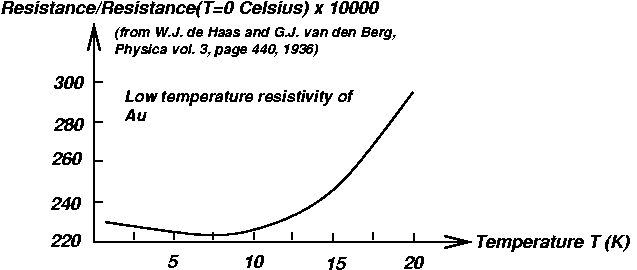
\includegraphics[scale=0.6]{/mnt/d/共享文件夹/毕设论文/latex模板/figures/Classickondo.png}
    \caption{含有少量铁杂质的金在低温下的行为}
    \label{fig}
\end{figure}
电阻率$\rho$在考虑了近藤效应后对温度T的依赖关系,如下
$$
\rho(T)=\rho_{0}+a T^{2}+c_{m} \ln \frac{\mu}{T}+b T^{5}
$$
其中$\rho_0$表示剩余电阻率,$aT^2$表示费米液体性质的贡献,$bT^5$表示晶格振动:$a,b,c_m$和$\mu$是与温度无关的量。近藤俊彦导出了第三项,该项与温度和实验观察到的呈对数关系。





\section{\ce{Ce3(Pt/Pd)In11}重费米子物理体系}
\subsection{超导与反铁磁共存}
迄今为止研究的大多数铈重费米子化合物都有 一个Ce离子的晶体学位点。在两个或者更多不等位点的化合物中,相应Ce离子的不同的局部环境导致Ce的4f轨道态与周围的配合基和传导态的不同相互 作用。这反过来导致不同的近藤耦合强度。因此,在这些多位点铈化合物中,可能会出现各种新的和复杂的现象,其中基态的特征在于不同电子和磁性状态在微观尺度上的共存。如图\ref{fig1},\ce{Ce3PdIn11}拥有两个Ce不等位点,其中一个Ce位点表示出顺磁性($T_N \approx 0.3K$)而另一个Ce位点展现反铁磁性($T_Q \approx 0.5K$)。

\begin{figure}[h]
    \centering
    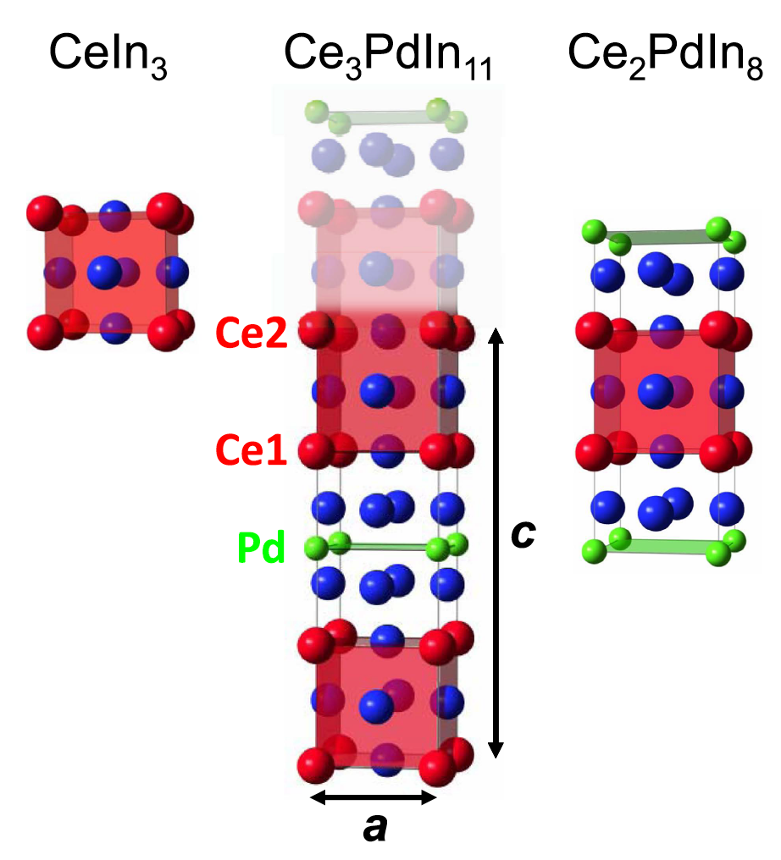
\includegraphics[scale=0.6]{/mnt/d/共享文件夹/毕设论文/latex模板/figures/figure 1.png}
    \caption{\Songti 图为\ce{Ce3PdIn11}的晶格结构(中间),指出了Ce两个不等位点Ce1和Ce2}
    \label{fig1}
\end{figure}


\ce{Ce3PdIn11}和\ce{Ce3PtIn11}都属于\ce{Ce_nT_mIn_{3n+2m}}类材料。包括了\ce{CeCoIn5}、\ce{CeRhIn8}和\ce{Ce2\\RhIn8}等一系列化合物。当Pd被Pt代替\ce{Ce3PdIn11}和\ce{Ce3PtIn11}晶体结构相似。在室温下的晶格常数分别是$a=4.687(4)$\AA 和$c=16.8422(12)$\AA。

同样\ce{Ce3PtIn11}也拥有两个不等位点,晶胞中的三个Ce离子分布在晶体学上不等价的位点内。两个Ce离子位于Ce1的位置,其被类似于\ce{Ce2PtIn8}中的Ce离子的配体包围。Ce2的位置被一个Ce离子占据,离子拥有类似\ce{CeIn3}的环境。在无磁场的情况下,\ce{Ce3PtIn11}在$T_1 \simeq 2.2K$和$T_N \simeq 2K$处经历两次连续的变化,进入反铁磁状态(AFM),并在$T_c \simeq 0.32K$以下变为超导。

\subsection{特性介绍}
\subsubsection{电阻率随温度变化}
如图\ref{fig2}在300K时,c轴电阻率等于$600 \Omega cm$,大约是基平面$\rho$的1.5倍。随着温度降低$\rho$表现出随温度$d \rho /d t > 0$的弱相关性。低于30K电阻率下降很快标志着高温下的不连续近藤散射向低温下的重电子布洛赫态的变化的交叉点。

\begin{figure}[h]
    \centering
    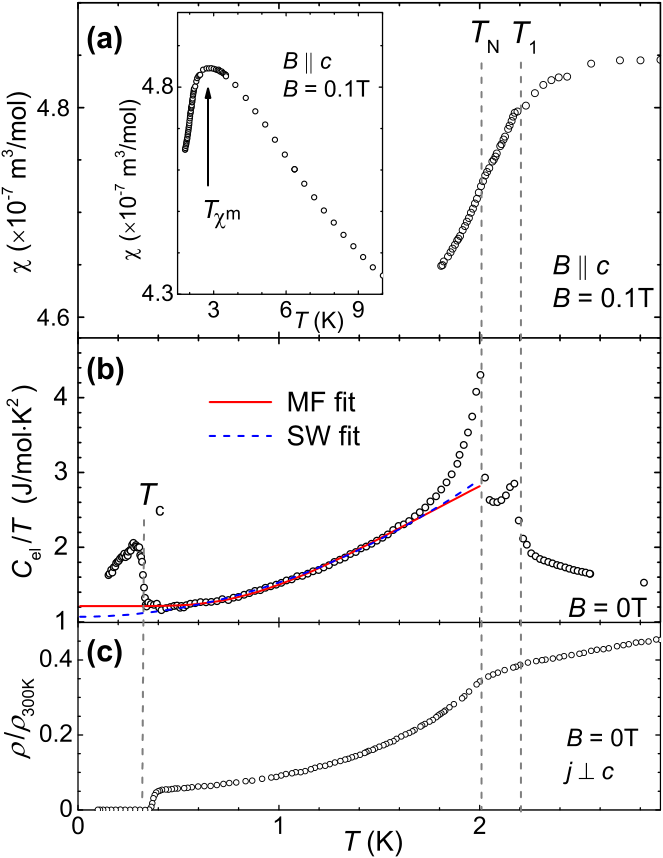
\includegraphics[scale=0.4]{/mnt/d/共享文件夹/毕设论文/latex模板/figures/figure4.png}
    \caption{概述了\ce{Ce3PtIn11}在$T < 3K$时的低温 特性。(a)在施加于c轴$B = 0.1T$的磁场中$\chi$与T的相关性。插入的部分显示了温度数据最大是10K。箭头指出了$\chi T$的最大值。(b)电子部分的比热$C_el/T$作为T的函数在零场中。红色的实线和蓝色的虚线分 别是$T < 0.8T_N$到$T = 0$的一个均值场和自旋波的拟合。(c)电阻归一化到其室温的值在B=0T和$j\perp c$。}
    \label{fig2}
\end{figure}

\subsubsection{磁化系数}
磁化系数作为温度的函数,$\chi(T)$沿晶格c轴和垂直于晶格c轴的磁场中测量到具有弱各向异性,在温度为3K时$\chi^{\parallel c}/\chi^{\perp c} \approx 1.25$。在超过150K时$\chi(T)$遵循Curie-Weiss定律两个方向的有效磁矩为$\mu_{eff}=2.60\mu_B /Ce$,与洪特规则对自由\ce{Ce^{3+}}离子符合很好。Weiss温度由对$\theta^{\perp c}_{p}=-64K$和$\theta^{\parallel c}_p=-42K$的曲线拟合到。图\ref{fig2}显示了\ce{Ce3PtIn11}在低温下的环境压力热力学和传输特性。在图\ref{fig2}(a)插入显示了在一个大的温度范围低温下磁化率$\chi^{\parallel c}$。

\subsubsection{反铁磁和非常规超导}
图\ref{fig2}a在更低温下$\chi(T)$在$T_1$时急剧下降,第二个AFM转变在$T \simeq 2.0k$表现为0.1T数据中显示为弱凸状结构。

将$C_{el}/T$跳跃的重点定义为过渡温度,分别得到$T_1 \simeq 2.2K$和$T_N \simeq 2K$,这些值与$\chi(T)$和$\rho(T)$的特征符合的很好(图\ref{fig2}中的虚线)。当$T=0.35K$时$C_{el}/T$发生了明显的变化,这表示了电阻率数据证实了材料向超导相的转变。将这个跳跃中点定义为$T_c \simeq 0.32K$。

为了估算通常比热系数$\gamma_n$外推AFM低温向$T=0$变化的尾部[图\ref{fig2}b红色虚线部分]采用二阶平均场类型表达式,$C_{el}/T=\gamma_n + A e^{-\Delta_{AFM}/T}$。拟合结果是$\gamma_n=1.21J/(molK^2)$,$A=8.97J/(molK^2)$和$\Delta_{AFM}=3.44K$(拟合区间是$0.44<T<1.6K$)。拟合$C_{el}/T \propto T^2$(AFM自旋波)描述了相同区间的数据,具有相似的质量,但是$\gamma_n$减小了大约10\%。使用上述参数可以计算参数$\Delta C/(\gamma T_c)\approx 0.7$,大约是BCS理论预期值的一半。我们可以在这里假设,参与超导的导带中的电子等量得来自两个Ce位点。







\section{反铁磁性和非常规超导共存和竞争机制}%分别介绍
\subsection{非常规超导简介}
在极低温下一些材料表现出完全抗磁性以及零电阻情况,常规超导可以用BCS(B\\ardeen-Cooper-Schrieffer)理论解释其中的微观图像,电子形成库伯对,配对电子可以凝聚,形成一个相位相干的宏观量子态。由此我们可以得到超导的共性:(1)常规材料的电子声子耦合较弱,转变温度$T_c$比较低;(2)超导态的序参量(超导电流密度)的对称性和晶格保持一致。超导态有广泛的应用前景,但是受限于较低转变温度$T_c$,难以大范围应用。

但是要提高$T_c$就得改变电子配对方式,对非常规超导尤其是重费米子超导体的研究表明,电子确实可以通过多种关联效应引起的临界涨落配对,比如自旋涨落、电荷密度涨落、价态涨落等,这些涨落足够强时,可以像声子一样在电子对之间产生净吸引效应,而克服电子之间的库伦排斥力并产生超导现象。并且大量的实验数据证实,无论是是从能量尺度还是对称性角度,非常规超导和量子相变往往是一起的。
\subsubsection{超导与反铁磁的竞争与共存}
重费米子超导的一个重要研究价值在其丰富的相图,如图\ref{fig3}所示,大部分材料的低温相图与铜氧化合物、铁基高温超导体又非常类似,如图\ref{fig3}c所示。但是最早发现Ce基超导的\ce{CeCu2Si2}仍然存在争议,从其相图看,材料中的超导和反铁磁序是竞争关系而非共存。可以简单理解为Ce原子的仅有的一个f电子很难同时参与反铁磁长程有序和超导序,但是并不妨碍反铁磁涨落与超导的共存关系。

2011年O.Stockert等人通过非弹性中子散射实验给出了反铁磁涨落驱动\ce{CeCu2Si2}超导的明确证据。在超导态,自旋激发能谱中看到了清晰的能隙,这由于磁交换能部分转变成了库伯对的凝聚能。同时在\ce{CeCu2Si2}、\ce{CePd2Si2}、\ce{CeAu2Si2}等材料都在高压下、反铁磁消失的边界区域出现超导相,暗示了超导与反铁磁相的竞争关系。



\begin{figure}[h]
    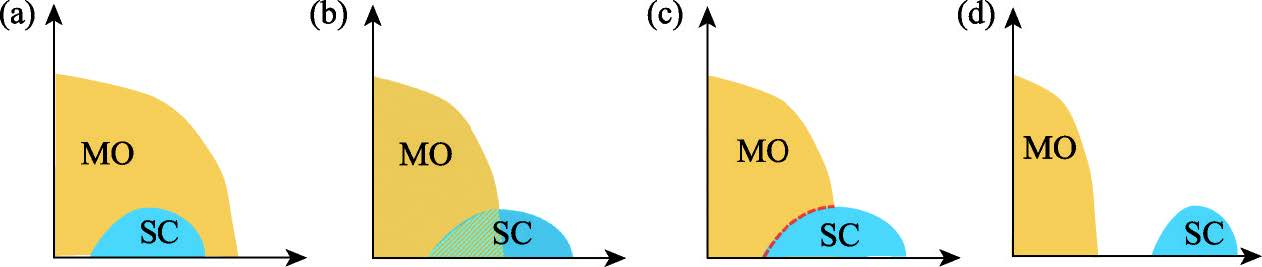
\includegraphics[scale=1.3]{/mnt/d/共享文件夹/毕设论文/latex模板/figures/figure5.jpg}
    \caption{重费米子超导体中超导相(SC)与磁有序相(MO)的竞争/共存相图,横坐标为化学掺 杂/替代、压力、偏压等调控手段,纵坐标为温度。(a)代表超导态完全处于磁有序相内 部,如 \ce{UGe2},\ce{YbRh2Si2} 等;(b)和(c)代表超导相从磁有序区域延伸到无磁性区域,但是(b)中超导与磁性可以在微观共存,如 \ce{CeRhIn5}、\ce{CePt3Si}、\ce{URhGe}、\ce{UCoGe}、(Ba,K)\ce{Fe2As2}、\ce{Ba(Fe,Co)2As2}等,而很多的 Ce 基、铜氧化合物、铁基超导体的相图与(c)一致;(d)代表 远离磁有序相以后材料才会出现超导态,比如 Pu-基超导体、\ce{CeCu2Si2}的高压超导相、\ce{\beta-YbAlB4} 等,价态涨落可能与这些材料的超导有关}
    \label{fig3}
\end{figure}

在2000年前后,发现的\ce{CeMIn5}(M=Co,Rh,Ir)极大的拓展了我们对重费米子超导以及反铁磁量子临界行为的认识。它们化学性质的特点在于Co、Rh、Ir这三种元素可以互相替代,获得连续可调的反铁磁态和超导态,同时超导和反铁磁相可以在微观共存。在\ce{CeRhIn5}中,电子的自旋和电荷自由度通过Kondo效应和RKKY相互作用紧密联系在一起,在图\ref{fig4}中可以明显看到温度-压力-磁场相图中很好的反应出来。
\begin{figure}[h]
    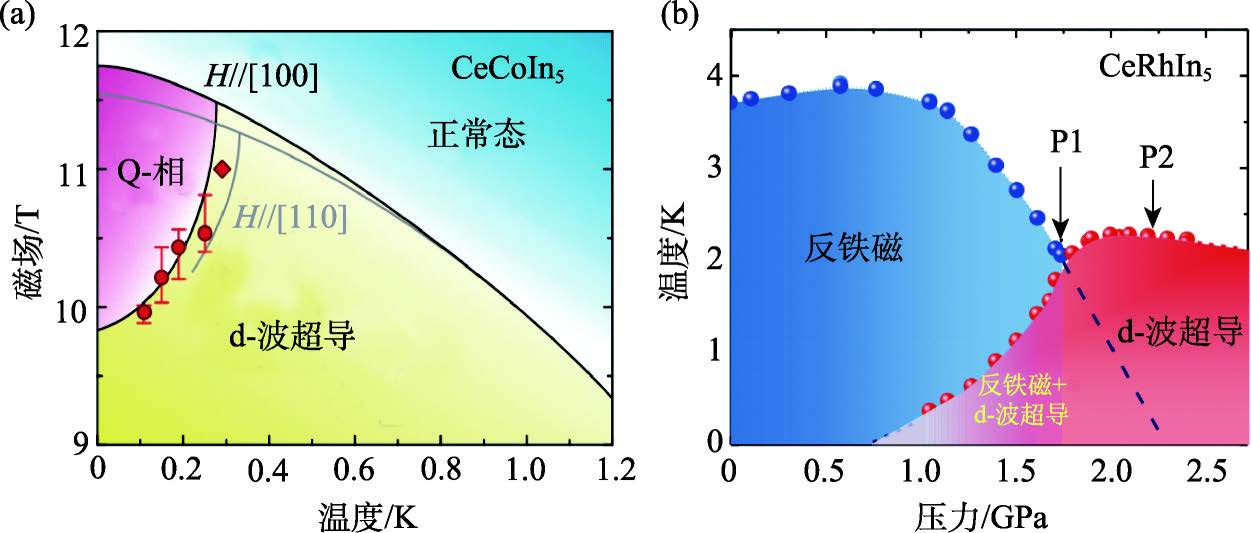
\includegraphics[scale=1]{/mnt/d/共享文件夹/毕设论文/latex模板/figures/figure6.jpg}
    \caption{(a)\ce{CeCoIn5}磁场温度相图,高磁场下粉红色区域为Q-相;(b)\ce{CeCoIn5}的压力-温度相图,中间粉色区域为超导与反铁磁共存的相}
    \label{fig4}
\end{figure}









\section{利用多体计算方法模拟安德森模型的初步结果}
\subsection{模拟结果数据处理程序的编写}

由于我们计算结果都存放在远程服务器上,所以我们在本地编写数据处理程序来帮助我们处理数据。
\subsubsection{运行所需环境}
我们的编写环境在Macos以及Linux下,程序语言是python,如下是需要的运行python库,其中pexpect库无法在Windows环境下运行,需要安装WSL2。
\begin{lstlisting}
    import pexpect
    from pathlib import Path
    import os
    import matplotlib.pyplot as plt
    import re
\end{lstlisting}

\subsubsection{程序编写思路}
我们将数据从服务器下载到本地处理,利用pexpect库向终端提交scp命令将数据打包下载到本地处理。
\begin{lstlisting}
    cmdline = 'scp -r %s %s@%s:%s' % (filename, user, ip, dst_path)
\end{lstlisting}
接着我们定义了四个函数利用字符串格式化匹配数据文件名
\begin{lstlisting}
def filename_U4(self, V1_value, V2s_value, Nsite, seed, T, mus):
    return "U4_V{}_tp{}_N{}_be{}_{}_mu{}.out".format(V1_value, V2s_value, Nsite, T, seed, mus)

def filename_local_orb(self, V1_value, V2s_value, Nsite, seed,T,mus):
    return "local_orb_U4_V{}_tp{}_N{}_be{}_{}_mu{}".format(V1_value, V2s_value, Nsite, T,seed, mus)

def filename_U4_tdm(self, V1_value, V2s_value, Nsite, seed,T, mus):
    return "U4_V{}_tp{}_N{}_be{}_{}_mu{}.tdm.out".format(V1_value, V2s_value, Nsite,T,seed, mus)

def filename_geom(self,V1_value,V2s_value,Nsite):
    return "geomU4_V{}_tp{}_N{}".format(V1_value,V2s_value,Nsite)
\end{lstlisting}
在获取文件名后利用python读取文件数据,进行字符串匹配,例如输出对.out文件的数据输出如下,返回数据存放在列表中。
\begin{lstlisting}
def data_out(self, path,filename, strs, numstart, numend):#输出结果
    data_list=[]
    a=[]
    b=[]
    with open(filename, 'r') as f:
        for i in f.readlines():
            data_list.append(i)
    for i in range(numstart,numend):
            k =data_list[i]
            result = "".join(k.split())
            a.append(result)
    for j in range(len(a)):
        if strs in a[j]:
            data_analysis.data_write(self,path,'result',data_list[j+numstart])
            b.append(data_list[j+numstart])
    return b
\end{lstlisting}
最后如下所示代码通过matplotlib库以及通过正则表达式对数据进行整合输出成图表,并且由于是面对对象的编程,本程序完成编写后可以为其他的程序调用,减轻了数据处理的负担。
\begin{lstlisting}
def data_temperature(self,path,ls,dtaus,V1_value,V2s_value,Nstie,\\ seed,mus,file):
    b=[]
    x=[]
    l=[]
    y=[]
    y0=[]
    err=[]
    y0err=[]
    for i in range(len(ls)):
        b.append(ls[i]*dtaus[i])
        x.append(1/(ls[i]*dtaus[i]))
    path1 = data_analysis.mkdir(self, path, V1_value, V2s_value, Nsite,mus)  # 创建文件夹返回路径
    path3 = path1 + '/' + file
    for k in b:
        filename_tdm=data_analysis.filename_U4_tdm(self,V1_value,V2s_value,\\ Nsite,seed,k,mus)
        if data_analysis.exit(self,path3,filename_tdm)==True:
            print('exit',filename_tdm)
        else:
            print("don't exit:",filename_tdm)
            data_analysis.download(self, '10.10.8.74', 'zhumo', '/home/zhumo/run_Ce3PtIn11/test', path1)
        l.append(data_analysis.data_tdm_out(self,path3,path3+'/'+
        filename_tdm,'Pd'))
    for i in l:
        p=re.findall(r"\d+\.?\d*",i[0])
        negative_p=re.findall(r"-\d+\.?\d*",i[0])
        print(p,negative_p)
        y.append(float(p[2])*10**float(p[3]))
        err.append(float(p[4])*10**float(negative_p[0]))
        y0.append(float(p[6])*10**float(p[7]))
        y0err.append(float(p[8])*10**float(negative_p[1]))
    plt.figure()
    plt.errorbar(x,y,yerr=err,fmt='-co')
    plt.errorbar(x,y0,yerr=y0err,fmt=',',ecolor='b',capsize=3)
    plt.xlabel('T')
    plt.ylabel('Pd_Pd0')
    plt.title(str(V1_value)+'-'+str(V2s_value),fontsize=12)
    plt.legend(title=('Pd','Pd0'))
    plt.ylim(0,0.5)
    # plt.xlim(0,30)
    plt.show()
\end{lstlisting}



\subsection{反铁磁结构因子}
我们使用DQMC对PAM模型的反铁磁结构因子进行验证。利用图\ref{fig5}(b)进行验证。其中参数如下
\begin{lstlisting}
V1_value = 1.0
V2s_value = 1.0
V12s=0.005
Ncell=6
Nsite=Ncell**2
ls=[20,40,60,80,100,120]
dtaus=[0.1,0.1,0.1,0.1,0.1,0.1]
T=ls*dtaus
seed='s1234567'
mus=0.0
\end{lstlisting}


\begin{figure*}[htbp]
    \centering
    \begin{minipage}[t]{0.4\textwidth}
    \centering
    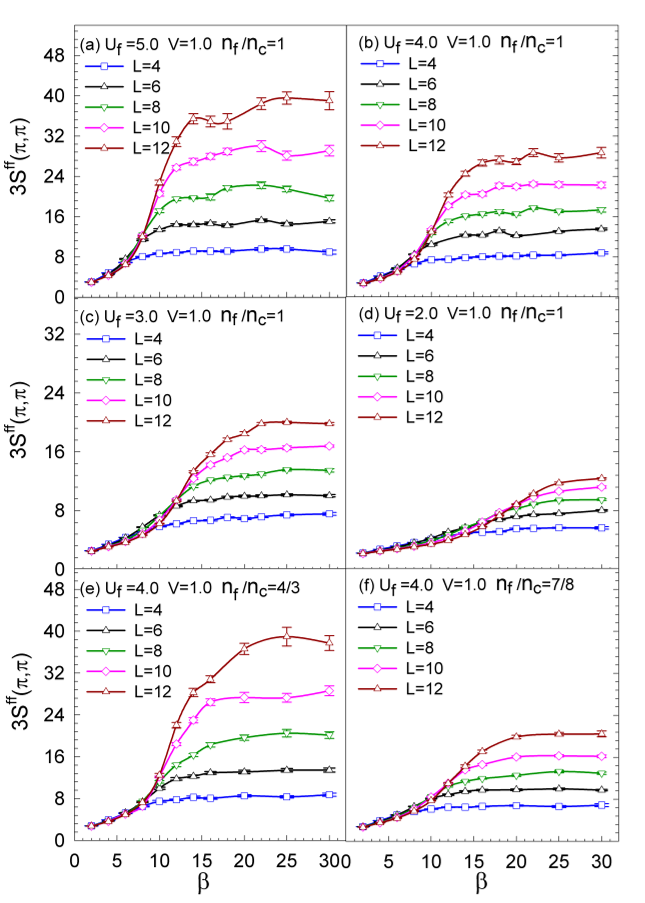
\includegraphics[scale=0.3]{/mnt/d/共享文件夹/毕设论文/latex模板/figures/figure3.png}
    \caption{(a)-(d)展示了在V=1时随着$\beta$的增加以及不同晶格大小的情况下AF结构因子的变化。}
    \label{fig5}
    \end{minipage}
    \begin{minipage}[t]{0.4\textwidth}
    \centering
    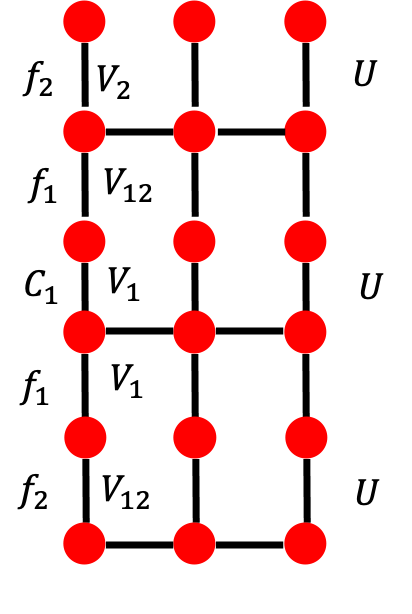
\includegraphics[scale=0.7]{/mnt/d/共享文件夹/毕设论文/latex模板/figures/figure2.png}
    \caption{简化后的计算模型}
    \label{fig6}
    \end{minipage}   
\end{figure*}


\begin{figure}[h]
    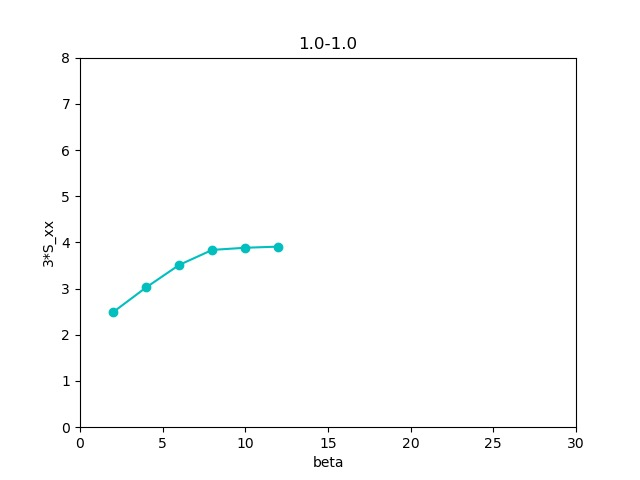
\includegraphics[scale=0.5]{/mnt/d/共享文件夹/毕设论文/latex模板/figures/figure7.jpg}
    \caption{横坐标$\beta=1/T$,而纵坐标为反铁磁结构因子。}
    \label{fig7}
\end{figure}

其中V1\_value是图\ref{fig6}中的$V_1$,同理V2s\_value是图\ref{fig6}中的$V_2$。通过服务器的模拟结果如图\ref{fig7}所示。与文献中符合的较好。


\subsection{超导计算结果}
利用DQMC计算二维Hubbard模型的超导相,以下是设置参数
\begin{lstlisting}
    V1_value = 1.0
    V2s_value = 0.001
    V12s=0.001
    Ncell=4
    Nsite=Ncell**2
    ls=[20,40,60,80,100,120]
    dtaus=[0.1,0.1,0.1,0.1,0.1,0.1]
    T=ls*dtaus
    seed='s1234567'
    mus=0.0
\end{lstlisting}
\begin{figure}[H]
    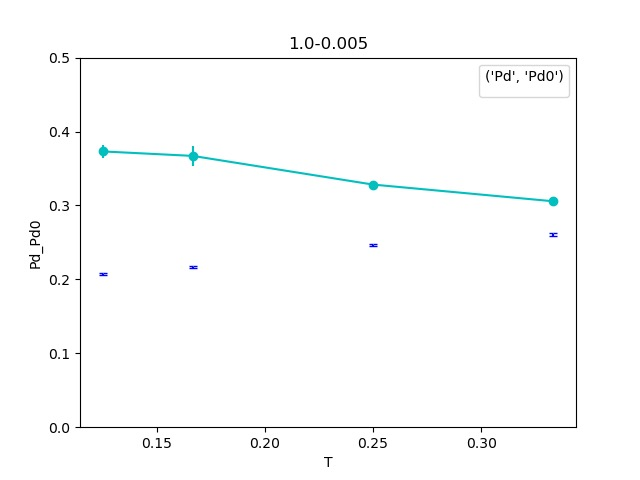
\includegraphics[scale=0.3]{/mnt/d/共享文件夹/毕设论文/latex模板/figures/figure9.jpg}
    \caption{不同温度下Pd和$\mathbf{Pd_0}$的趋势图(紫色为$Pd_0$,蓝色为Pd)}
    \label{fig9}
\end{figure}

\begin{figure}[H]
    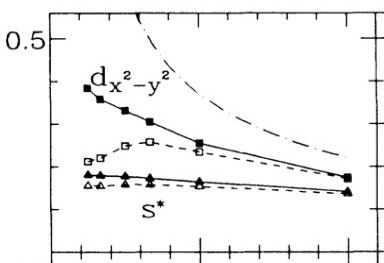
\includegraphics[scale=0.5]{/mnt/d/共享文件夹/毕设论文/latex模板/figures/figure8.jpg}
    \caption{在半填充($\left \langle n \right \rangle=1$)下,绘制了不同对场模式下对场磁化率P(实心点)和不相关对场磁化率P(空心点)与T的关系图。}
    \label{fig8}
\end{figure}

利用图\ref{fig8}验证结果正确性,计算结果如图\ref{fig9}所示。



























\newpage

%=================== 结论 ===============
% E 结论

\section{总结与展望}
\subsection{总结}
首先我们介绍了\ce{Ce3(Pd/Pt)In11},这种重费米子材料可以允许反铁磁和非常规超导的共存,并且两者还有竞争与共存机制,通过对这类材料的研究能够加深我们对重费米子材料超导机制的理解。并且我们对Hubbard模型近似,通过设置合适的参数,利用DQMC对周期安德森模型进行了模拟,与文献的结果符合较好。并且初步完成了对Hubbard模型的计算模拟,初步验证了在\ce{Ce3(Pd/Pt)In11}中超导和反铁磁的机制。

同时我们我们利用python对计算结果进行处理,成功实现了数据的自动化处理,极大方便了后期的数据备份以及分析。

\subsection{未来展望}
我们计划进一步通过设置参数利用DQMC对Hubbard模型进行进一步模拟,将\ce{Ce3(Pd/Pt)In11}材料中的超导与反铁磁共存与竞争机制通过计算机模拟出来。

对于反铁磁与超导态在微观上是如何相互耦合的,我们目前还没能很好的解释,也是我们未来的研究方向。

同样对于重费米子材料的研究,例如非常规超导的测量以及调控,能够拓展我们对强关联物理的理解,并且由于重费米子材料中的相互作用比较复杂,目前还未形成一个朴实的模型。目前主要有唯象自旋涨落理论、涨落交换近似理论、轨道选择理论、自洽重整化理论等多种理解思路。重费米子材料在当前的科学研究中发挥着重要作用

\newpage

%==================== 参考文献 ===========
% F 参考文献
\begin{thebibliography}{20}
\addcontentsline{toc}{section}{参考文献}
\bibitem{1} Kratochvílová M, Prokleška J, Uhlířová K, et al. Coexistence of antiferromagnetism and superconductivity in heavy fermion cerium compound Ce3PdIn11[J]. Scientific reports, 2015, 5(1): 1-11.
\bibitem{2} Wu W, Tremblay A M S. d-wave superconductivity in the frustrated two-dimensional periodic Anderson model[J]. Physical Review X, 2015, 5(1): 011019.
\bibitem{3} Prokleška J, Kratochvílová M, Uhlířová K, et al. Magnetism, superconductivity, and quantum criticality in the multisite cerium heavy-fermion compound Ce 3 PtIn 11[J]. Physical Review B, 2015, 92(16): 161114.
\bibitem{4} Custers J, Diviši M, Kratochvílová M. Quantum critical behavior and superconductivity in new multi-site cerium heavy fermion compound Ce3PtIn11[C]//Journal of Physics: Conference Series. IOP Publishing, 2016, 683(1): 012005.
\bibitem{5} Das D, Gnida D, Bochenek Ł, et al. Magnetic field driven complex phase diagram of antiferromagnetic heavy-fermion superconductor Ce3PtIn11[6]. Scientific Reports, 2018, 8(1): 1-10.
\bibitem{shi20180702} Kambe S, Sakai H, Tokunaga Y, et al. In 115 NQR study with evidence for two magnetic quantum critical points in dual Ce site superconductor Ce 3 PtIn 11[J]. Physical Review B, 2020, 101(8): 081103.
\bibitem{7} Fukazawa H, Kumeda K, Shioda N, et al. Successive magnetic transitions in the heavy-fermion superconductor Ce 3 PtIn 11 studied by In 115 nuclear quadrupole resonance[J]. Physical Review B, 2020, 102(16): 165124.
%\bibitem{DLWPfull} Eli. Stevens and Luca. Antiga, Deep Learning with PyTorch[M]. Manning Publications Co.
\bibitem{8} Shioda N, Kumeda K, Fukazawa H, et al. Determination of the magnetic q vectors in the heavy fermion superconductor Ce 3 PtIn 11[J]. Physical Review B, 2021, 104(24): 245119.
\bibitem{9} 沈斌, 袁辉球. 磁性量子相变[J]. 物理, 2020, 49(9): 570-578.
\bibitem{10} De Haas W J, Van Den Berg G J. The electrical resistance of gold and silver at low temperatures[J]. Physica, 1936, 3(6): 440-449.
\bibitem{11} 李正中. 固体理论[M]. 高等敎育出版社, 2002.
\bibitem{12} Zhang L, Ma T, Costa N C, et al. Determinant quantum Monte Carlo study of exhaustion in the periodic Anderson model[J]. Physical Review B, 2019, 99(19): 195147.
\bibitem{13} White S R, Scalapino D J, Sugar R L, et al. Attractive and repulsive pairing interaction vertices for the two-dimensional Hubbard model[J]. Physical Review B, 1989, 39(1): 839.
\end{thebibliography}

\newpage

%==================== 致谢  =============
% G 致谢
\section*{致谢}
\addcontentsline{toc}{section}{致谢}

感谢在苏大的四年,四年时间过得很快,还记得刚刚进入苏大校园懵懂的我,现在已经快要毕业并且即将迈入人生的下一个阶段。

回想这四年,从大一一路磕磕绊绊走来,苏大校园承载了太多回忆:和队友通宵赶实验进度的物科楼,期末奋战过的鸿远楼,考研时常去的本部图书馆,常去聚餐的莉莉小炒。

很庆幸这在苏大的四年没有荒废,一路走来高中还在求学的同学已经寥寥,很感谢大学室友能够激励我走到现在。

很感谢本科的指导过我的老师,翁雨燕老师,董裕力老师还有杨俊义老师,感谢你们的栽培,因为在本科期间能够让我尝试到不同方向的项目,我才能找到自己感兴趣的研究方向。同时也感谢毕业论文的指导老师蒋密老师,虽然毕设我只接触了短短的一两个月,但是在这过程中我学到了很多,虽然没能继续强关联方向的学习,但是所学到的知识在之后的科研和工作中必定受益终身。

感谢这一路走来帮助过的我的辅导员郭永坤老师,帮我解决了生活学习上大大小小的问题,感谢我的爸爸妈妈,没有他们我无法幸福得度过这人生中最好的四年。

愿各位前程似锦,养天地正气,法古今完人。


\newpage

%==================== 附录 ===============
% H 附录 (符号说明,原始材料等)
\section*{附录}
\addcontentsline{toc}{section}{附录}

\begin{description}
    \item 
    以下是本文所用到的数据处理程序,编写语言为python,运行环境为macOS和Linux。
	\begin{lstlisting}
		
import pexpect
from pathlib import Path
import os
import matplotlib.pyplot as plt
import re

class data_analysis(object):

    def __init__(self):
        self.passwd_key = '12345'#密码
        print("data_analysis Working")

    def upload(self, ip, user, dst_path, filename):
        # 上传
        cmdline = 'scp -r %s %s@%s:%s' % (filename, user, ip, dst_path)
        try:
            child = pexpect.spawn(cmdline)
            child.expect(self.passwd_key)
            child.sendline()
            child.expect(pexpect.EOF)
            print("file upload Finish!")
        except Exception as e:
            print("upload failed:", e)

    def download(self, ip, user, dst_path, filename):
        # 下载
        cmdline = 'scp -r %s@%s:%s %s' % (user, ip, dst_path, filename)
        try:
            child = pexpect.spawn(cmdline)
            child.expect("password")
            child.sendline('12345')
            child.expect(pexpect.EOF, timeout=None)  #timeout是持续时间如果下载时间很长可以大一点
            print("file download Finish!")
        except Exception as e:
            print("download failed:", e)

    def exit(self, path, filename):#判断文件是否存在
        p = Path(path)
        if p.is_dir() == True:
            files = p.glob(filename)
            if len(list(files)) == 0:
                print('dont exit')
                return False
            else:
                print('exit')
                return True
        else:
            print("this isn't a dir")

    def data_write(self,path,filename,data):
        with open(path+'/'+filename+'.txt','a+') as f:
            f.writelines(data+'\n')
        print('write success')

    def data_out(self, path,filename, strs, numstart, numend):#输出结果
        data_list=[]
        a=[]
        b=[]
        with open(filename, 'r') as f:
            for i in f.readlines():
                data_list.append(i)
        for i in range(numstart,numend):
                k =data_list[i]
                result = "".join(k.split())
                a.append(result)
        for j in range(len(a)):
            if strs in a[j]:
                data_analysis.data_write(self,path,'result',\\ data_list[j+numstart])
                b.append(data_list[j+numstart])
        return b

    def data_out_local(self,path,filename, strs, numstart,numend):#local_orb文件结果输出
        data_list=[]
        a=[]
        b=[]
        with open(filename, 'r') as f:
            for i in f.readlines():
                data_list.append(i)
        for i in range(numstart,numend):
                k =data_list[i]
                result = "".join(k.split())
                a.append(result)
        for j in range(len(a)):
            if str(a[j]).startswith(strs)==True :
                data_analysis.data_write(self,path,'result',data_list\\ [j+numstart])
                b.append(data_list[j+numstart])
        return b


    def data_tdm_out(self,path,filename,strs):
        data_list=[]
        a=[]
        b=[]
        with open(filename, 'r') as f:
            for i in f.readlines():
                data_list.append(i)
        for i in range(len(data_list)):
                k =data_list[i]
                result = "".join(k.split())
                a.append(result)
        for j in range(len(a)):
            if str(a[j]).startswith(strs)==True:
                for o in range(15):
                    data_analysis.data_write(self,path,'result',\\ data_list[j+o])
                    b.append(data_list[j])
                break
        return b


    def mkdir(self,path,V1_value,V2s_value,Nsite,mus):#创建文件夹
        Path=path+'/'+str(V1_value)+'_'+str(V2s_value)+'_'+str\\ (Nsite)+'_'+str(mus)
        folder = os.path.exists(Path)
        if not folder:
            os.makedirs(Path)
            return Path
        else:
            return Path



    def filename_U4(self, V1_value, V2s_value, Nsite, seed, T, mus):
        return "U4_V{}_tp{}_N{}_be{}_{}_mu{}.out".format(V1_value, V2s_value, Nsite, T, seed, mus)

    def filename_local_orb(self, V1_value, V2s_value, Nsite, seed,T,mus):
        return "local_orb_U4_V{}_tp{}_N{}_be{}_{}_mu{}".format(V1_value, V2s_value, Nsite, T,seed, mus)

    def filename_U4_tdm(self, V1_value, V2s_value, Nsite, seed,T, mus):
        return "U4_V{}_tp{}_N{}_be{}_{}_mu{}.tdm.out".format(V1_value, V2s_value, Nsite,T,seed, mus)

    def filename_geom(self,V1_value,V2s_value,Nsite):
        return "geomU4_V{}_tp{}_N{}".format(V1_value,V2s_value,Nsite)

    def data_conclusion(self,path,V1_value,V2s_value,Nsite,seed,\\ T,mus,file):
        filename_judge = data_analysis.filename_U4(self,V1_value, V2s_value, Nsite, seed, T,mus)  # U4文件名
        filename_local_orb = data_analysis.filename_local_orb(self,V1_value, V2s_value, Nsite, seed, T,mus)  # local_orb文件名
        filename_geo = data_analysis.filename_geom(self,V1_value, V2s_value, Nsite)
        filename_tdm = data_analysis.filename_U4_tdm(self,V1_value, V2s_value, Nsite,seed,T,mus)
        path1 = data_analysis.mkdir(self,path, V1_value, V2s_value, Nsite)  # 创建文件夹返回路径
        path3=path1+'/'+file
        if data_analysis.exit(self,path3, filename_judge) == True and data_analysis.exit(self,path3, filename_local_orb) == True and data_analysis.exit(self,path3, filename_geo) == True and data_analysis.exit(self,path3, filename_tdm) == True:
            data_analysis.data_write(self,path1, 'result', '=============================')
            data_analysis.data_write(self,path1, 'result', 'Avg and Density')
            data_analysis.data_out(self,path1, path3 + '/' + filename_judge, 'Avg', 1, 47)
            data_analysis.data_out(self,path1, path3 + '/' + filename_judge, 'Density', 1, 47)
            data_analysis.data_write(self,path1, 'result', 'local_orb')
            strs = ['11', '22', '33', '44', '55', '66']
            for k in strs:
                data_analysis.data_out_local(self,path1, path3 + '/' + filename_local_orb, k, 23, 59)
            data_analysis.data_write(self,path1, 'result', 'Hamilt')
            data_analysis.data_out(self,path1, path3 + '/' + filename_geo, '', 17, 35)
            data_analysis.data_write(self,path1, 'result', 'tdm_out')
            data_analysis.data_tdm_out(self,path1, path3 + '/' + filename_tdm, 'Pd')
        else:
            data_analysis.download(self,'10.10.8.74', 'zhumo', '/home/zhumo/run_Ce3PtIn11/test', path1)
            Path2 = path1 + '/' + file
            data_analysis.data_write(self,path1, 'result', '=============================')
            data_analysis.data_write(self,path1, 'result', 'Hamilt')
            data_analysis.data_out(self,path1, Path2 + '/' + filename_judge, 'Avg', 1, 47)
            data_analysis.data_out(self,path1, Path2 + '/' + filename_judge, 'Density', 1, 47)
            data_analysis.data_write(self,path1, 'result', 'local_orb')
            strs = ['11', '22', '33', '44', '55', '66']
            for k in strs:
                data_analysis.data_out_local(self,path1, Path2 + '/' + filename_local_orb, k, 23, 59)
            data_analysis.data_write(self,path1, 'result', 'Hamilt')
            data_analysis.data_out(self,path1, Path2 + '/' + filename_geo, '', 17, 35)
            data_analysis.data_write(self,path1, 'result', 'tdm_out')
            data_analysis.data_tdm_out(self,path1, path3 + '/' + filename_tdm, 'Pd')
        return 'Finish'

    def data_temperature(self,path,ls,dtaus,V1_value,V2s_value,Nstie,\\ seed,mus,file):
        b=[]
        x=[]
        l=[]
        y=[]
        y0=[]
        err=[]
        y0err=[]
        for i in range(len(ls)):
            b.append(ls[i]*dtaus[i])
            x.append(1/(ls[i]*dtaus[i]))
        path1 = data_analysis.mkdir(self, path, V1_value, V2s_value, Nsite,mus)  # 创建文件夹返回路径
        path3 = path1 + '/' + file
        for k in b:
            filename_tdm=data_analysis.filename_U4_tdm(self,V1_value,\\ V2s_value,Nsite,seed,k,mus)
            if data_analysis.exit(self,path3,filename_tdm)==True:
                print('exit',filename_tdm)
            else:
                print("don't exit:",filename_tdm)
                data_analysis.download(self, '10.10.8.74', 'zhumo', '/home/zhumo/run_Ce3PtIn11/test', path1)
            l.append(data_analysis.data_tdm_out(self,path3,\\ path3+'/'+filename_tdm,'Pd'))
        for i in l:
            p=re.findall(r"\d+\.?\d*",i[0])
            negative_p=re.findall(r"-\d+\.?\d*",i[0])
            print(p,negative_p)
            y.append(float(p[2])*10**float(p[3]))
            err.append(float(p[4])*10**float(negative_p[0]))
            y0.append(float(p[6])*10**float(p[7]))
            y0err.append(float(p[8])*10**float(negative_p[1]))
        plt.figure()
        plt.errorbar(x,y,yerr=err,fmt='-co')
        plt.errorbar(x,y0,yerr=y0err,fmt=',',ecolor='b',capsize=3)
        plt.xlabel('T')
        plt.ylabel('Pd_Pd0')
        plt.title(str(V1_value)+'-'+str(V2s_value),fontsize=12)
        plt.legend(title=('Pd','Pd0'))
        plt.ylim(0,0.5)
        # plt.xlim(0,30)
        plt.show()
    #
    # def data_out_tdm(self,path,ls,dtaus,V1_value,V2s_value,Nstie,\\ seed,mus,file):
    #     return True






path = '/Users/xbunax/Documents/dqmc/dqmc_T'  # 文件夹地址
V1_value =1.0
V2s_value = 1.0
Ncell=4
Nsite=Ncell**2
ls=[20,40,60,80,100,120]
dtaus=[0.1,0.1,0.1,0.1,0.1,0.1]
file='dqmc_T'
#T=ls*dtaus
seed='s1234567'
mus=[0.0]
#data_analysis.data_conclusion(data_analysis,path,V1_value,\\ V2s_value, Nsite,seed,T,number)
data_analysis.data_temperature(data_analysis,path, ls, dtaus, V1_value, V2s_value, Nsite, seed, mus,file)





	\end{lstlisting}
\end{description}


\end{document}

